\chapter{The SAFE Network}
\label{ch:thesafenetwork}

Decentralisation of data is the core benefit of the SAFE Network. As with many things in life, once someone has ownership or control of something they can either use that position of power for good purposes or for less desirable ones. The internet as it exists today is very fragile in this regard. When you upload a file to Dropbox\cite{dropbox} or OneDrive\cite{onedrive}, where does this file exist? Well that file exists solely on the servers that those organisations have control over. Once an organisation has data they can do with it what they please, acting within the bounds of overcomplicated privacy polices to manage your data. Not only does this incur the obvious privacy infringements (which we will not cover cover too much within this paper), but it can lead someone into the false sense of security that their data is safe. If for instance, someone managed to hack Dropbox or there was a catastrophic failure at the datacenter, who is to say that your data would be safe? That would depend upon a lot of factors such as: do they keep backups, do you yourself have a local copy of the file etc. On a much larger scale companies like Amazon provide AWS\cite{amazon-aws}, an enterprise grade cloud-computing platform. If AWS were to fail, or be targeted, many of the worlds biggest websites would cease to function. This is because this computational power, data is centralised. It is not necessarily an \textit{easy} target, but it is a single identifiable piece of the equation that if removed, causes the whole thing to collapse. This \textit{problem} is what the SAFE Network means to answer and is a question I will be exploring throughout this paper.

\subsection{Ownership of Data on the SAFE Network}

Accessing the SAFE Network is \textit{permission-less}. What this means is that you don't need to go to a central body that controls the network to ask for (register) an account. You simply connect to the network and create one yourself. This has big implications for how people can interact with the network. Once you establish a connection to the network and create an account, you have the same exact same rights and privileges as any other user on the network. You can retrieve any data that exists on the network (although you may not have the cryptographic keys to actually read that data) and store data if you have enough Safecoin. Safecoin is the \textit{cryptocurrency} of the SAFE Network, it is used to pay for the storage of data and to reward nodes for storing data\cite{lambert2015safecoin}. I will go into much further depth later on in the paper. Once a user has enough Safecoin, they can store any arbitrary data on the network that they wish. They can either make this data public, for instance sharing a photograph, or encrypt this data and do with the key what they wish. At a high level, an account is just a piece of data that is stored on the network. It is made up of an \textit{Account Secret} and a \textit{Account Password}. With both of these you can log into the network and interact with all the data you have uploaded to the network. Your \textit{Account Secret} and \textit{Account Password} never leave your client, they are not stored anywhere and are never sent in plaintext to the network (again I will explain this in much greater detail later). This means that \textbf{only} the person who has access to \textbf{both} the \textit{Account Secret} and the \textit{Account Password} can: see what data the account has written to the network, manage the privileges to the data and decrypt any data the account has used its encryption keys for.

In decentralised data storage networks, who owns the data is a difficult question to answer. The example we will examine is BitTorrent\cite{cohen2008bittorrent}. The SAFE Network shares some core characteristics with BitTorrent but deviates greatly on some others. The \textit{ownership} of data is one such point. In BitTorrent (and other decentralised data storage networks) who actually \textit{owns} the data. Is it the person who uploaded the torrent or is it collectively owned by everyone who holds a copy of that data? In the SAFE Network, the ownership of data is more clearly defined. When data is uploaded to the SAFE Network, the data is split up into chunks and distributed across nodes that makeup the network. The data is duplicated across different nodes (which introduces a level of redundancy) and is available for consumption by anyone who has the key to that data. If it was uploaded as \textit{public} data then anyone (with the correct address) can read that data. Fundamentally though, that data has an owner. The account that originally uploaded it to the network. They can do with it what they wish, including deleting the data permanently. This contrasts with BitTorrent greatly, wherein data cannot simply be \textit{deleted}. If you shared data on BitTorrent then wanted to delete it, you would have to communicate directly to each client that had a copy of the data and ask them to delete it. They do not have to comply with this request. Thus the SAFE Network having the concept of \textit{ownership of data} is very important as it opens up different use cases that haven't existed before.

Owing to this system of ownership, it brings about its own challenges in regards to the law. Data that has been written to the network is \textit{immutable} without the \textit{Account Secret} and \textit{Account Password}. It cannot be removed or deleted. This could mean that users could simply upload copyrighted/illicit material to the network as public, delete their \textit{Account Secret} and \textit{Account Password} and it will be available to everyone forever. Even if the original uploader was apprehended, they couldn't even delete the data if they wanted to as they have forgotten the necessary login to do so. This system is a natural consequence of the design of the SAFE Network. You cannot have a permission-less and decentralised data storage network that has a \textit{master-key} to alter data. To do so would undermine the security of the network as a whole, if such a key existed then bad parties would eventually discover it. A key concept is that users control their own data. Nobody else. If such a \textit{master-key} existed then this property of the SAFE Network would be \textit{broken} and its use cases diminished dramatically. Thus the uploading and distribution of illegal or copyrighted content could be a huge issue for the adoption of the SAFE Network. I have spent a great deal of time pondering this question, I see it as the biggest challenge the SAFE Network will have to overcome. People \textbf{will} use it to distribute copyrighted and illegal content, the SAFE Network is essentially the \textit{perfect} system to do so. This problem \textbf{will} become evident when the SAFE Network reaches full release. The biggest issue is user perception, take Tor\cite{tor} as an example. Many people in the general populous think of the 'Dark Web'\cite{dark-web} as a haven for all kinds of illicit activity. Thus when they hear of applications like Tor that can be used to access the 'Dark Web' they make this association. "Tor means illicit activity". This same problem \textbf{will} exist for the SAFE Network. I feel it is very important that Maidsafe realise this and take the proper precautions to educate people. At the end of the day, the SAFE Network is a tool. Like any other tool, people will most likely do bad things with it. The difficult question to answer is if the benefit it provides to \textit{good} people justify the benefits it provides to \textit{bad} people.
 
\section{Peer to Peer vs Client Server}

Centralisation of data and computing power is a natural consequence of the Client-Server architecture that has formed around the internet. Throughout this section, I will use \textit{Netflix}\cite{netflix} as an example to help illustrate my points. When you watch a video on Netflix, your device is merely a consumer of that data. A server owned by Netflix streams the video to your device and that is as far as the relationship goes. With this architecture, there are some obvious benefits. Mainly for the realm of rights management. As Netflix controls access to the data it holds (in this case video files) it is \textit{easy} for them to regulate access to it. They have complete control over what happens to that data. Let's contrast this with another, very popular, means of consuming video that works using a Peer-To-Peer architecture. Figure \ref{fig:client-server-peer2peer} shows a Client Server network and a Peer to Peer network.

\begin{figure}
	\begin{center}
		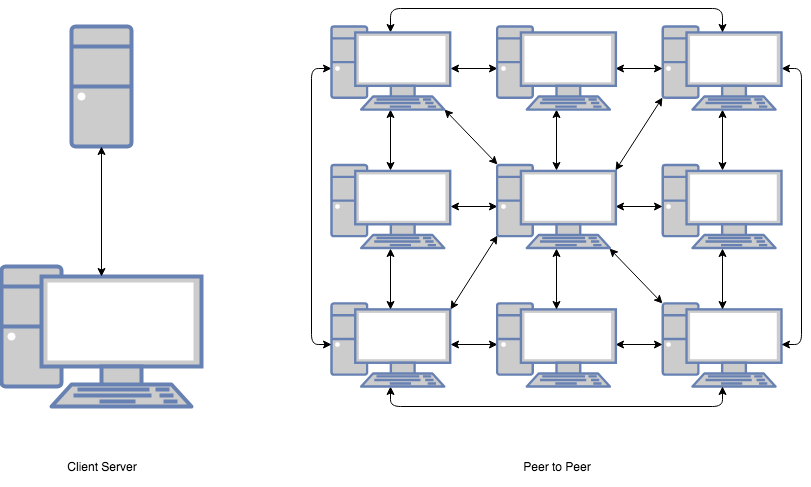
\includegraphics[width=\textwidth]{diagrams/client-server-vs-p2p}
		\caption{Client-Server vs Peer-to-Peer Network}
		\label{fig:client-server-peer2peer}
	\end{center}
\end{figure}

\subsection{BitTorrent}

The first stable version of the BitTorrent protocol was released in 2001. Since then it has become one of the worlds most popular means of file sharing and indeed internet traffic. Accounting for \%3.5 of global internet traffic at the time of writing\cite{bittorrent-usage}. In a \textit{permission-less} environment users are allowed to freely share files with one another. As there is no centralised body controlling who has access to what data, the system has been widely used for the \textit{piracy} of copyrighted material. The BitTorrent protocol helps to solve many of the same challenges that the SAFE Network aims to. One of which is the centralisation of data in a Client-Server architecture. In the BitTorrent protocol, peers form what is known as a 'swarm'. A 'swarm' is all clients that aim to download a a full copy of a piece of data. A piece of data is broken down into chunks and each chunk has a unique hash that allows clients to uniquely identify each piece of the original file. A client in the swarm is referred to as \textit{peer} when they don't have all the relevant pieces of a file. A client in the swarm is referred to as a \textit{seed} when they do hold all pieces of a given file. The 'resting state' of this network is when all clients in the swarm are \textit{seeds}. So clients will use peer-to-peer routing to send chunks of the file to other clients in the swarm that do not have it. This way of sharing data brings about many benefits. 

In BitTorrent there is no central 'server' to attack (disregarding a \textit{tracker}, there are \textit{tracker-less} solutions available). This means that you can lose clients from the swarm (or clients can leave and rejoin) and as long as at least one person in the swarm has a copy of a specific chunk of data all clients in the swarm can spread the data and become \textit{seeders}. This level of data redundancy is a huge benefit to BitTorrent over a traditional client-server model. You can see the topology of a tracker based swarm in Figure \ref{fig:bittorrent-tracker}.

\begin{figure}
	\begin{center}
		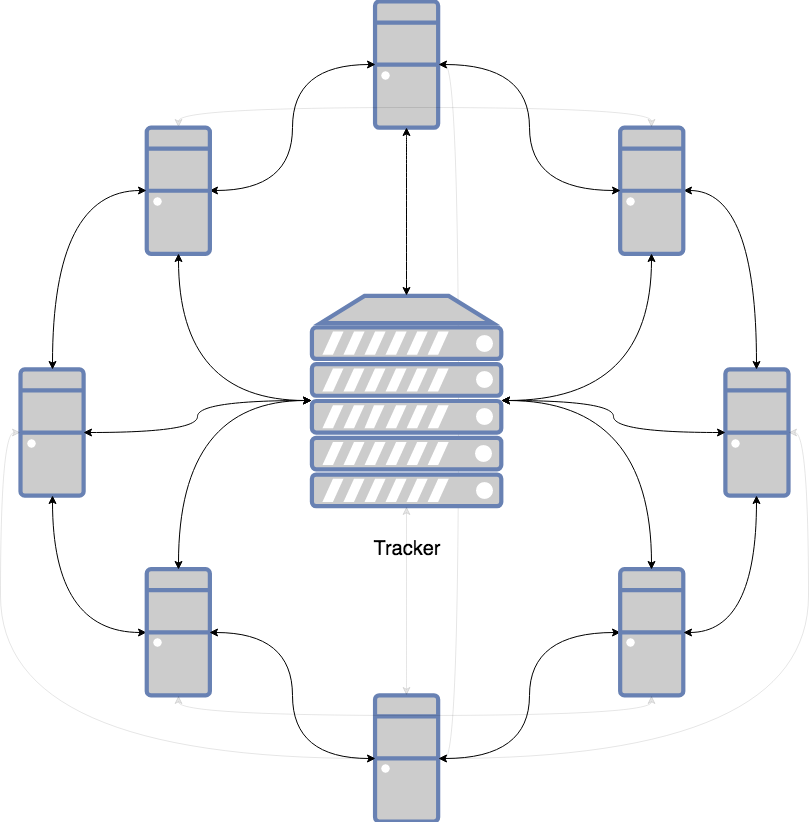
\includegraphics[scale=0.3]{diagrams/bittorrent}
		\caption{Topology of tracker based swarm in BitTorrent}
		\label{fig:bittorrent-tracker}
	\end{center}
\end{figure}

Data transfer costs are also a huge benefit to BitTorrent. In the traditional model, the owner of the server has incurs great cost in the hosting of the file. They have to pay for the management, storage and the network costs of sharing that data. For large companies this is often a negligible cost that doesn't impact on them, for smaller organisations however (especially non-profits) this server cost can be a big problem. This is a big reason why many Linux distributions so often provide BitTorrent links to download the operating system. By using BitTorrent they can offload the cost of sharing the file onto their users. This works almost on a good-samaritan basis. Where in if you download a file you really should aim to have your \textit{seed-ratio} hit at least 1 before leaving the swarm permanently (a clients \textit{seed-ratio} is how much of the file they serve to other users against how much they themselves have downloaded from the swarm). For the vast majority of users this cost is negligible and can act as a 'good-will' gesture to help support projects.

Data transfer speeds are a major positive of the BitTorrent protocol. When a client is acting as a \textit{peer}, their download speed is limited to the summation of the upload speeds of the clients they are receiving file chunks from. This means that in a well established swarm that your file will download as fast as your internet connection will allow. The more users that join the swarm, the faster and more resilient to failures the network gets.

This might all sound wonderful, but there is a glaring \textit{flaw} that means that companies like Netflix cannot use BitTorrent to offload network responsibilities to its users. That \textit{flaw} is control. Once shared, a video file cannot be easily removed from the network. This has big implications for things like Copyright, where they may only have the licence to provide access to a piece of content for a set period of time. I use the term \textit{flaw} very usefully, many people would indicate that this is one of BitTorrent's biggest benefits and I would agree with them. It is however important to realise that this is a limiting factor to organisations who could otherwise find use in the technology.

BitTorrent may solve many issues surrounding the distribution of files, but falls short of solving the decentralisation of the internet as a whole. The main limitation attributing to this is that data on BitTorrent is not mutable. Once a file has been spread to a swarm it is an immutable entity that cannot be changed. This limits BitTorrent to the sharing of files and not being able to do things like support dynamic websites, forums, email etc. (I want to emphasis that I don't mean this as a criticism of BitTorrent. It does one thing and does it very well. It has a proven track record of working and has laid the groundwork for other projects, such as the SAFE Network). The other attributing factor is that data only exists inside \textit{swarms}, you cannot interact with data without first joining the relevant swarm. So the discoverability of data is an issue. A given node within the network can't work out how to retrieve a chunk of data that is not located in the swarms it belongs to. These are all points that the SAFE Network aims to address.

\subsection{Serverless Architecture}

The idea behind a serverless architecture is to move as much computation/functionality to the client as possible. As time passes, the computational power that the masses have access to gets faster and faster. This computational power goes \textit{wasted} for the most part. When you browse the internet, interact with Facebook for instance, your computer actually does very little in terms of processing the information you are seeing. It does have to do work rendering websites and such but there is computational power going unused. Most, if not all, of the data is processed on FaceBooks' servers then merely served to you as a consumer. Your browser is a \textit{thin-client}. Not only does this incur vast operational costs for organisations, but it also means that information is being processed on their server that could be done locally.

In the SAFE Network, there are no 'servers' so to speak. The 'servers' on the network are what are called \textit{vaults}. I will give a deeper explanation of \textit{vaults} later in the report, for now just think of them as serving a similar purpose as to what nodes do in a BitTorrent swarm.  The only interaction a client has with the SAFE Network is the storage or retrieval of data, that it. So the SAFE Network in this capacity can serve a similar purpose to BitTorrent. Additionally what the SAFE Network has is the ability to route requests throughout the entire network. All \textit{vaults} in the network have knowledge of how to find a given chunk of data that exists on the network. This is different to BitTorrent because it can only find a chunk of data within the swarms it knows about. As this dynamic routing exists, the SAFE Network has a form of DNS that can be used. Another major difference is the SAFE Network is capable of mutable data. This means that the SAFE Network is fully capable of supporting dynamic websites, forums, email etc. You can open a browser that is capable of connectivity with the SAFE Network and browse the \textit{internet} just as you would normally. Only in this circumstance you are browsing an entire \textit{internet} supported by a Peer-To-Peer architecture.

At a high level, the only purpose a \textit{vault} serves is to store and serve data. That's it. This means that websites built for the SAFE Network must offload all the processing to the client and only use the network as its storage 'back-bone'. Thus the \textit{Serverless Architecture} model is a good fit for the SAFE Network. It allows you to build very powerful websites but keeps the processing of data local. This method of building websites has been around for a long time. With the advent of JavaScript and other such technologies, it was possible to dynamically change websites locally and run code locally without needing the server to do any processing. Very powerful JavaScript \textit{applications} can be served, think of online games. A website that serves these \textit{mini-games} doesn't do the processing for the game on their server. They merely serve the JavaScript/Flash/Java/Etc code to you and then your computer/client does all the hard work. Another of this are online \textit{office suites}, they are very powerful programs that can be ran through the browser. They depend heavily on the processing power of the user to provide them with an experience similar to what they could achieve with a desktop application. A true \textit{serverless architecture} model takes this to the extreme, there is absolutely no processing of data on the server. It is all done on the client. 

The way the SAFE Network operates forces the \textit{serverless architecture} architecture to be used (unless you merely use the SAFE Network as a component in your stack). This introduces challenges in that it is a new way of thinking about how to design websites and applications. Instead of complex servers, you almost entirely erase this concern from your development. You don't really need to consider how your apps data will be served, just how you go about accessing/storing it. Instead of designing websites the \textit{traditional} way, you develop them like you would a \textit{fat-client}. Websites will become heavier, requiring more care and optimisations. Messy and slow JS is abundant in the internet today, mostly due to the abundance of computing power that exists. Why spend time optimising when you can throw more CPU and RAM at it? This hap-hazard way of thinking cannot really exist for \textit{serverless architecture} websites or users will not have a great experience. An avenue that I think will become popular within the SAFE Network developer community is Web Assembly. 

Web Assembly is an assembly-like language that you can compile C, C++, Rust, etc, to and then run inside web browsers. It allows you to write code in high-level languages (that aren't interpreted like JS) and then serve it to users such that the code runs with \textit{near native} performance. This has big implications for the internet as a whole, not just the SAFE Network. A technology like Web Assembly could therefore be extremely useful when building websites that use the \textit{serverless architecture} model. It can give developers access to languages and frameworks to build websites that just weren't available before. As it promises near-native performance, it could be a great tool with which to build rich websites that aren't clunky and slow. Websites that run nearly as fast as desktop applications will therefore be possible.

\section{A Return to Fat Client Applications}

At a high-level, a \textit{Fat Client} is a computer (application) that can perform operations and tasks without relying on a central \textit{server}. A Fat Client may still need to make periodic connections to a server but the vast majority of its functionality can be performed without \textit{chatter} with the server. The concept of a Fat Client is juxtaposed to that of a Thin Client. Traditionally a Thin Client was a lightweight computer that relied heavily on a server to have any sort of utility. They would be able to perform some tasks locally but the vast majority would require a constant connection to a server. The traditional model of the internet, an overwhelmingly client-server based structure, has encouraged the growth of the Thin Client model. Historically this approach does make sense, computers were expensive and if you could centralise the required computational power you could reduce costs. In todays world however, computing power is fast and readily available. As discussed previously, this computational power (for the most part) goes to waste. Applications (specifically internet browsers) are acting as Thin Clients for content. Although not all Fat Clients follow the \textit{serverless architectural model}, applications that are designed to be \textit{serverless} are inherently Fat Clients. Hence because of the points mentioned previously, the SAFE Network encourages (almost requires) the Fat Client style of architecture.

This has vast implications for how applications should be designed for the SAFE Network and indeed influenced the choices I made for SAFE Wiki. Not only does one have to follow the design principles of the \textit{serverless architectural model}, but also that of the Fat Client. As Web Technologies grow, mature and develop it brings about new possibilities for how Fat Client applications can be used by end users. Instead of having to download applications to your device, new technologies allow rich \textit{serverless fat client} applications to be built and delivered through the web. A user simply needs to browse the internet as they already do instead of changing it to a model where they would have to download an app for Facebook, Twitter, YouTube etc. This style of \textit{content delivery} was not possible before, Web Technologies were not mature enough to support such rich experiences without relying heavily on server side processing. Hence I view the advent of new Web Technologies, such as Web Assembly that was mentioned above, to be an enabler in the success of the SAFE Network.

\subsection{An Example, Netflix on the SAFE Network}

Unlike BitTorrent, the SAFE Network could indeed be used to facilitate a service like Netflix. At its core, Netflix is about data. Their main goal being streaming the data that they have (video) to as many users around the world as possible and to do it as fast as possible. Although they would be able to benefit from redundancy and reduced server costs, there are flaws in the BitTorrent protocol that make it extremely difficult to justify it as a means of facilitating a website like Netflix. The biggest issue being ownership of data. As discussed previously, websites like Netflix have to have 'ownership of data'. They have to be able to control and \textit{mutate} the access of individuals to content. They simply cannot do this on BitTorrent. Another glaring whole in that approach is that of the health of the swarm. For content (data) to be available, nodes have to be online and sharing that file. This could mean that popular content would be readily \textit{seeded} but more obscure content may not be. The extreme of this being that the most obscure content might only be \textit{seeded} by Netflix themselves, resulting in a return to the Client-Server model they currently have. The SAFE Network solves these issues. Ownership of data is clearly defined, you own your data and nobody else does. Architecturally the SAFE Network insures that there are multiple copies of data spread around the network, meaning files will always be redundantly stored across the network. 

A Netflix style of service very much fits the \textit{Fat Client} style of architecture. Video playback is already processed locally so the content delivery system is the key part of the system that changes. Considerations to how things like 'Suggestions' would work are the biggest challenges in my opinion. Currently, that kind of feature fits the client server model quite well. Netflix gathers information about the shows you watch then suggests similar content that you might like to view. As this happens server side it is a continually updating entity that can improve and adapt, the inner-workings completely hidden from the user. With a \textit{serverless architectural} model this approach is simply unfeasible, There is no \textit{processing} of information on the SAFE Network. This would mean that to perform actions like 'content suggestion' you would have to perform it locally, client side. This applies to any application that is built on the SAFE Network. Users are quite used to visiting a service, such as Netflix or Facebook, and seeing newly \textit{generated} content that was created whilst their client was off. To account for this, new approaches in how to generate content will have to be thought of. This might be as simple as generating/processing the content when the user first opens the client and then displaying it to them. A more complicated approach might be to encourage users to keep applications open in the background so this processing can take place. In the browser this makes sense, users are familiar with the concept of keeping 'browser tabs' open. Often 'bookmarking' or 'favouriting' their favourite sites. One could envision a system wherein these 'tabs' would be refreshed in the background so users don't notice any delay when opening up the application (website). Traditional 'desktop' applications don't have this same luxury. Users typically 'quit' applications when not in use, so they would either need to be kept alive in the background (which may annoy some) or rely on quickly generating/processing content on startup.

\section{Alternative Business Models}

Like any new technology, the SAFE Network opens up many opportunities that didn't exist before. How the SAFE Network operates with \textit{Farming} and \textit{Safecoin} opens up new opportunities in how users could pay for content. In SAFE Network nomenclature, \textit{vaults} farm data. The safe and reliable storage (farming) of data is rewarded with \textit{Safecoin} which is a cryptocurrency built into the SAFE Network. One could envision an application that instead of charing users to use it, instead allows them to become a vault that generates Safecoin. This Safecoin could then be sent back to the creators of the program and hence financially compensates them for the usage of their application. A service like Netflix could very well make use of this kind of scheme, encouraging users to have their own vaults that then increases the performance of the network as a whole. One consideration of this approach however is that vaults don't get to choose what data they store, that is an integral part of the architecture of the SAFE Network. By following this financial model then it would be for the 'good of the whole', increasing the utility of the entire network and not just for one application.

This really is all about how to best use the processing power of the world. When a user sits and watches Netflix on an entertainment system, there is very little strain on the resources of the device. In the case of a games console, literally teraflops of processing power, advanced networking and storage facilities are going unused. Potential financial models can try to \textit{exploit} this untapped power to the benefit of both the user and the provider of the application. The most simple means I can see is to use that power to \textit{farm} \textit{Safecoin}. Not only increasing the utility of the SAFE Network but providing users with an entirely new way to pay for content. Offering the resources they have in exchange for access to services.

\section{Architecture of the SAFE Network}

The SAFE Network is still very much in active development. At the time of writing, the SAFE Network is currently on its second alpha revision (Alpha 2) out of a planned four. This not only made this project difficult because of a lack of documentation (I can't really blame them, it is not a 'finished' project), but means that anything I talk about in terms of the technicalities of the network is subject to change. In \textit{Chapter \ref{ch:architecture}} I will explain to the best of my ability how the network operates and functions \textbf{at the time of writing}. I don't expect much, if anything, to change in the near future. Just keep this in mind.
